\documentclass[letterpaper]{article}

\usepackage[english]{babel}
\usepackage[utf8]{inputenc}
\usepackage{amsmath}
\usepackage{graphicx}
\usepackage[colorinlistoftodos]{todonotes}
\usepackage[]{algorithm2e}
\usepackage{listings}
\usepackage{hyperref}
\usepackage{float}
\usepackage{afterpage}

\title{CSCE 636: Homework 2}

\author{Aryan Sharma\\UIN: 326006767} % The article author(s) - author affiliations need to be specified in the AUTHOR AFFILIATIONS block

\date{} % An optional date to appear under the author(s)

\begin{document}
	
\maketitle

\noindent {\Large Question 1}\\

\noindent \textbf{1a.} 	We need to flatten the data set loaded as the data that is loaded from MNIST are 2D images. We convert this to a vector because it makes the computation easier and also conveniently fits into the vectorized computation as required in tensorflow. \\

\noindent \textbf{1b.} Implemented in code\\

\noindent \textbf{1c.} Implemented in code\\

\noindent \textbf{1d.} Implemented in code\\

\noindent \textbf{1e.} Epoch was trained as the hyperparameter. The best setting came at epoch 9 with validation accuracy to be 97.74\%. \\

\noindent {\Large Question 2}\\

	\[
		\frac{\partial E_{in}}{\partial w} =  \frac{\partial}{\partial w} (\frac{1}{N} \sum_{n=1}^{N} (\tanh (\textbf{w}^T\textbf{x}_n) - y_n)^2)
	\]
	\[
		= \frac{2}{N} \sum_{n=1}^{N} (\tanh (\textbf{w}^T\textbf{x}_n) - y_n) \frac{\partial}{\partial w} (\tanh (\textbf{w}^T\textbf{x}_n) - y_n)
	\]
	\[
		= \frac{2}{N} \sum_{n=1}^{N} (\tanh (\textbf{w}^T\textbf{x}_n) - y_n) (1- \tanh^2 (\textbf{w}^T\textbf{x}_n)) \frac{\partial}{\partial w} (\textbf{w}^T\textbf{x}_n)
	\]
	\[
		= \frac{2}{N} \sum_{n=1}^{N} (\tanh (\textbf{w}^T\textbf{x}_n) - y_n) (1- \tanh^2 (\textbf{w}^T\textbf{x}_n)) \textbf{x}_n
	\]
	
	When the weights go to infinity, the gradient goes to 0. This exploding gradient problem would then cause the perceptron to always have large positive activation and thus would fail to classify negative data points. Also since the gradient is 0, no extra training iteration would update it's weight and bring down. This is a common problem in perceptron which classifies all the data points as positive when the gradient explodes. To solve this the model should have a regularization parameter. \\

\noindent {\Large Question 3}\\
	
	Given, the values we have,
	
	 \begin{figure} [H]
		\centering
		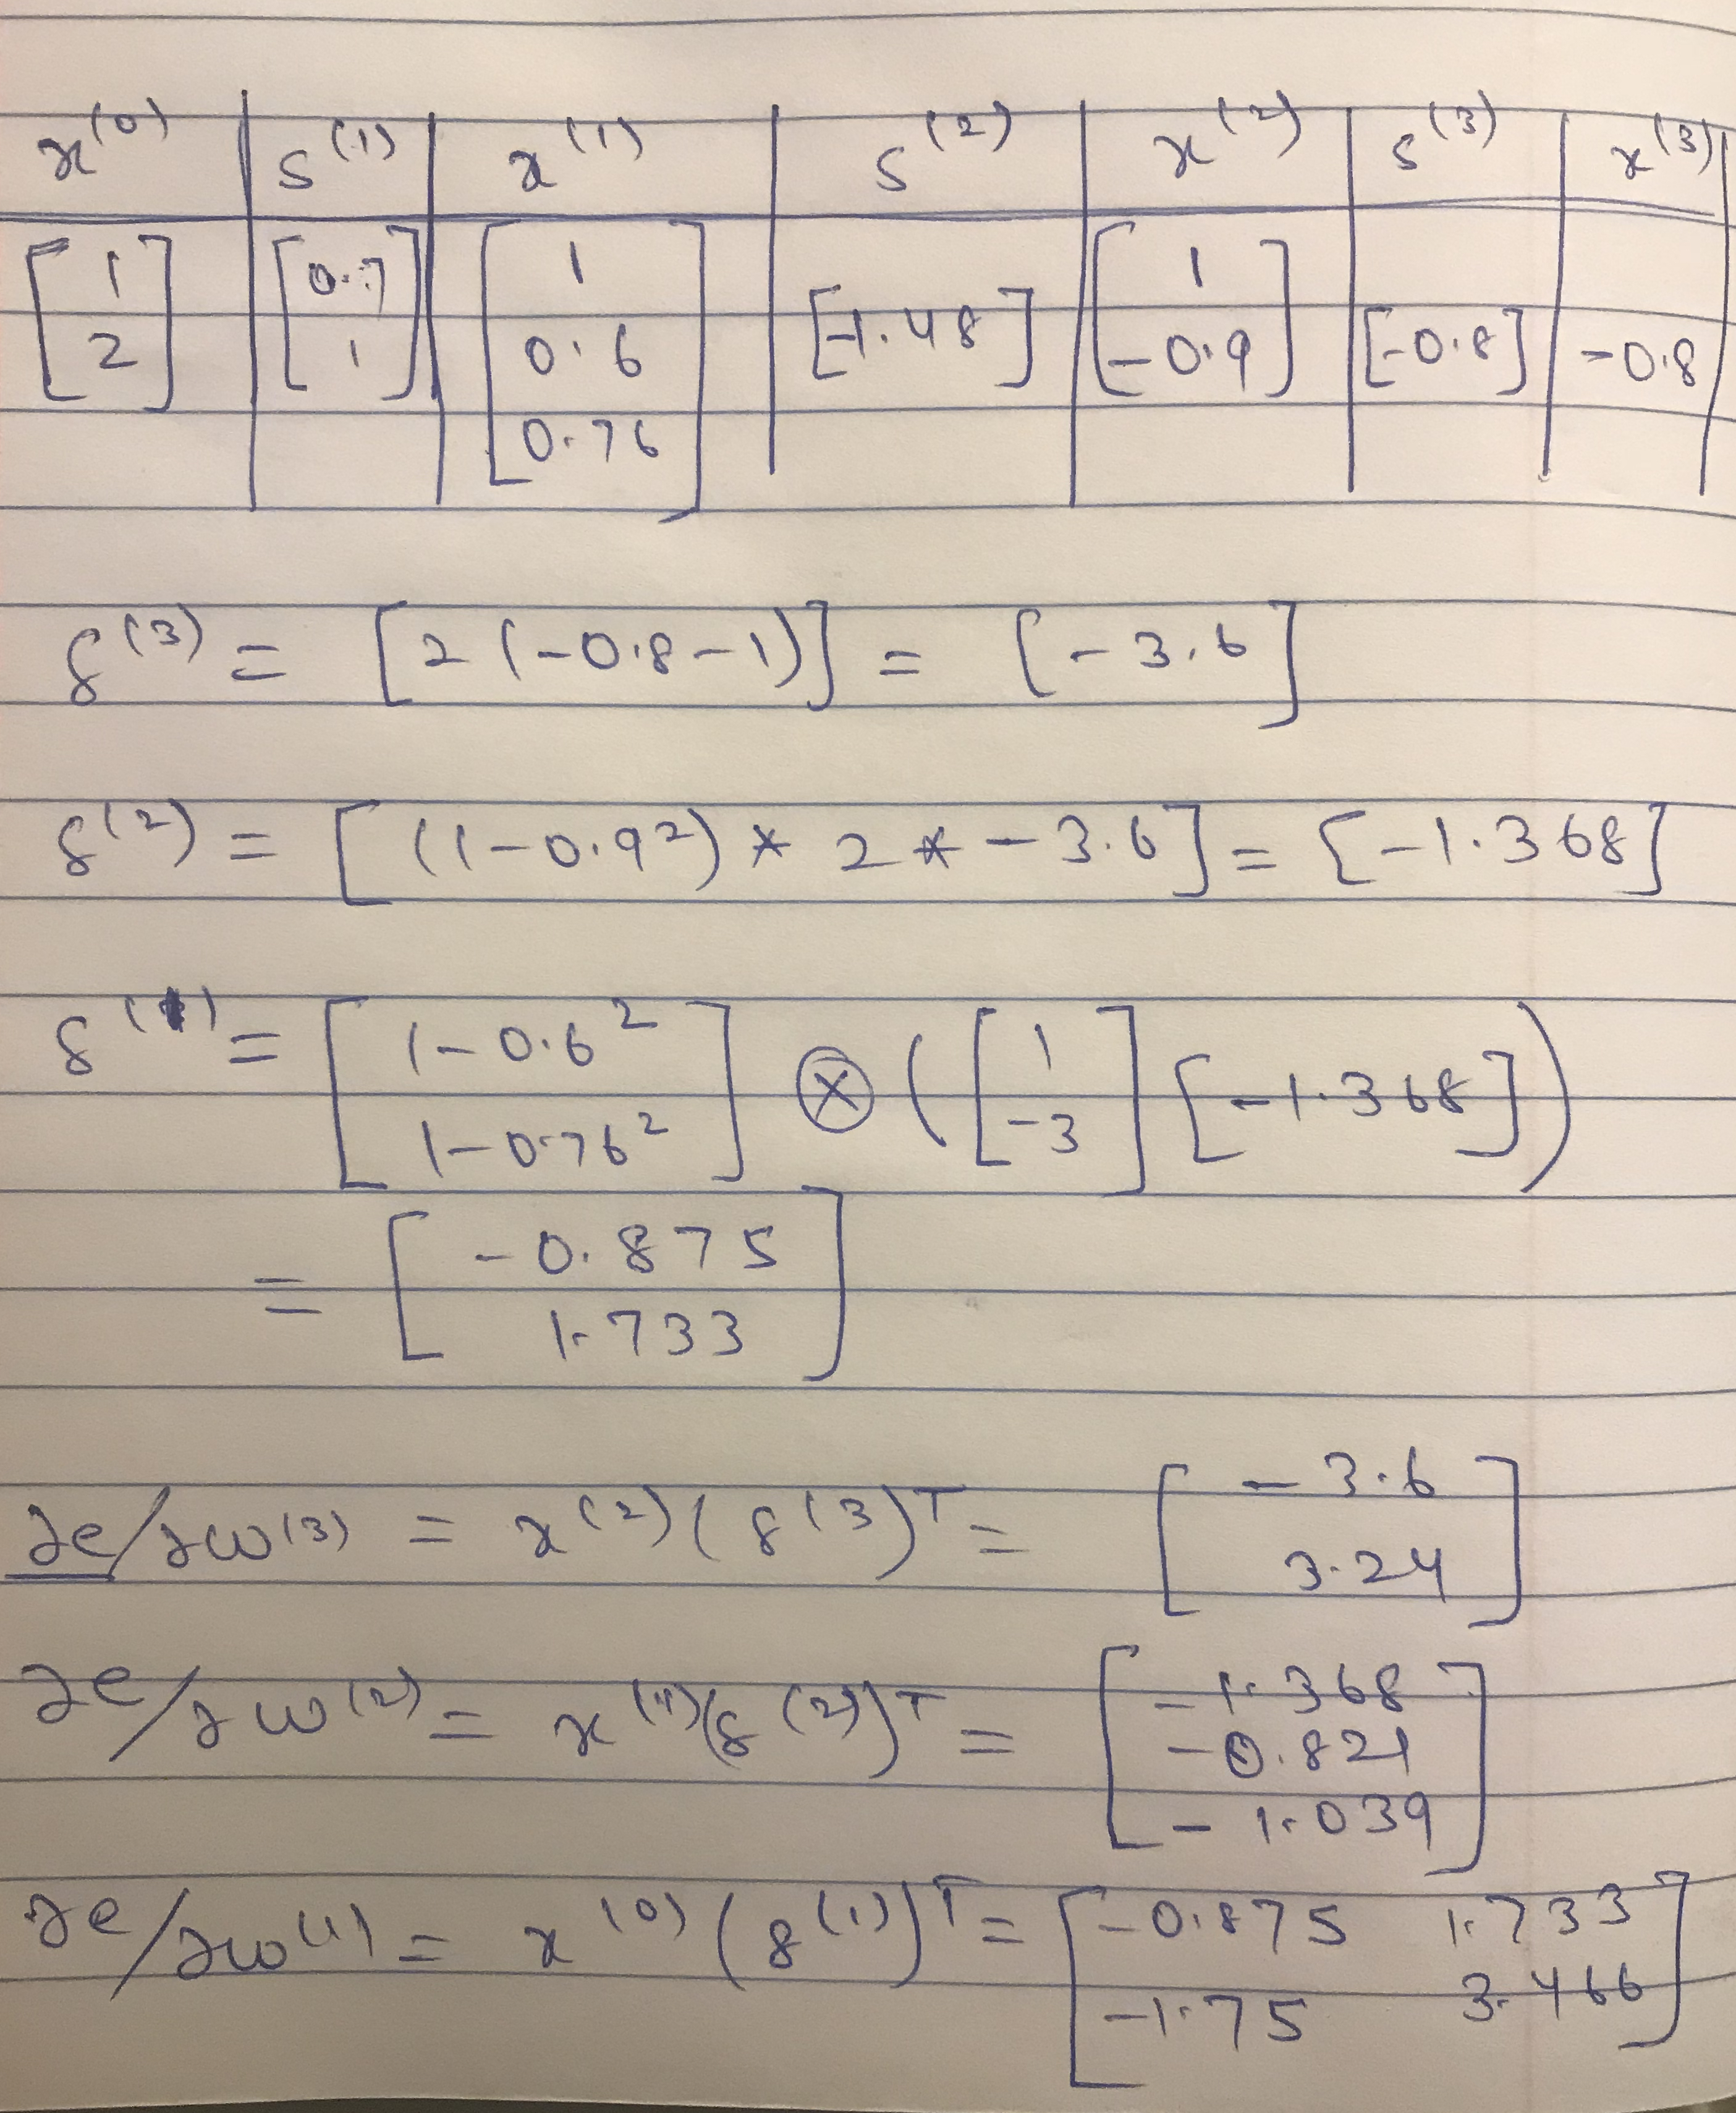
\includegraphics[width=0.8\textwidth]{img.jpg}
		\caption{\label{fig:data}Question 3}
	\end{figure}

\noindent {\Large Question 4}\\
	
	\noindent Given, 
	\[
		E(w) = (w - w^{\ast})^TQ(w-w^{\ast})
	\]
	\[
		\frac{\partial}{\partial w} E(w) = (Q + Q^T)(w-w^{\ast})
	\]
	Since \(Q\) is positive definite matrix,
	\[
		\frac{\partial}{\partial w} E(w) = (2Q)(w-w^{\ast})
		\tag{1}
	\]
	Putting \(w = 0\), we have 
	\[
		\frac{\partial}{\partial w} E(w) = -2Qw^{\ast}
	\]
	
	Setting Equation 1 to 0, we get the \(w = w^{*}\). Hence the optimal value is \(w^{*}\) and these are the weights that minimize \(w\).
	
	No, the gradient does not move in the direction of the optimal weights as when \(w\) is 0, we can see the gradient to negative when \(w^{\ast}\) is positive and positive otherwise. Hence, owing to the gradient, the optimization does not move in the correct direction.
	
	The more big the step the more oscillation it causes while reaching the optimal value. In cases with very high learning rate, it may diverge.
	
	
	

\end{document}